\documentclass[12pt]{article}

%Begin----------------------------------------------------------------------------------------------------------------------------------------
%---------------------------------------------------------------------------------------------------------------------------------------------


%Package import and Config of Packages
%\usepackage[utf8]{inputenc}%\usepackage{tikz}#
\usepackage{lmodern}
\usepackage{setspace}
\usepackage{lastpage}
\usepackage{pgfplots} % Fuer Plots
\usepackage{pgfplotstable}
\usepackage{pgfkeys} 
\usepackage{filecontents}
\pgfplotsset{compat = newest}
\usepackage{tikz} % Generell gutes Packet
\usepackage{csvsimple} % Zum CSV auslesen
\usepackage{fancyhdr}
\usepackage{tcolorbox}


\usepackage[ngerman]{babel}
\usepackage{datetime}
\newdateformat{myformat}{\THEDAY{ten }\monthname[\THEMONTH], \THEYEAR}


\usepackage{subfig}
\usepackage{pdfpages}
\usepackage{subfiles}
\usepackage{titlesec}
\usepackage[pdfborder={0 0 0}]{hyperref}
\usepackage{pdfpages}
\usepackage{verbatim}
\usepackage{geometry}
\geometry{left=20mm, right=20mm, bottom=20mm}

\usepackage{graphicx}
\graphicspath{{../Bilder/}{Bilder/}}

\usepackage{xcolor}
\usepackage{listings}
%End------------------------------------------------------------------------------------------------------------------------------------------
%---------------------------------------------------------------------------------------------------------------------------------------------
%Package import and Config of Packages

%Begin----------------------------------------------------------------------------------------------------------------------------------------
%---------------------------------------------------------------------------------------------------------------------------------------------
%List Configuration for Coding
\usepackage{listings} % Generell Code-Boxen
\usepackage{xcolor} % Fuer extra Farben mit color{}

\colorlet{punct}{red!60!black}
\definecolor{background}{HTML}{EEEEEE}
\definecolor{delim}{RGB}{20,105,176}
\colorlet{numb}{magenta!60!black}

\definecolor{mGreen}{rgb}{0,0.6,0}
\definecolor{mGray}{rgb}{0.5,0.5,0.5}
\definecolor{mPurple}{rgb}{0.58,0,0.82}
\definecolor{backgroundColour}{rgb}{255,255,255}

\lstdefinestyle{StyleVHDL}
{
    backgroundcolor=\color{backgroundColour},
    belowcaptionskip=1\baselineskip,
    breaklines=true,
    xleftmargin=\parindent,
    language=VHDL,
    frame = single,
    showstringspaces=false,
    basicstyle=\footnotesize\ttfamily,
    keywordstyle=\bfseries\color{magenta},
    commentstyle=\color{mGreen},
    identifierstyle=\color{blue},
    stringstyle=\color{orange},
}
\lstdefinestyle{StylePython}
{
    backgroundcolor=\color{backgroundColour},
    belowcaptionskip=1\baselineskip,
    breaklines=true,
    xleftmargin=\parindent,
    language=Python,
    frame = single,
    showstringspaces=false,
    basicstyle=\footnotesize\ttfamily,
    keywordstyle=\bfseries\color{magenta},
    commentstyle=\color{mGreen},
    identifierstyle=\color{blue},
    stringstyle=\color{orange},
} 
\lstdefinestyle{StyleMatlab}
{
  backgroundcolor=\color{backgroundColour},   
  belowcaptionskip=1\baselineskip,
  breaklines=true,
  xleftmargin=\parindent,
  language=Matlab,
  frame = single,
  showstringspaces=false,
  basicstyle=\footnotesize\ttfamily,
  keywordstyle=\bfseries\color{black},
  commentstyle=\color{mGreen},
  identifierstyle=\color{blue},
  stringstyle=\color{magenta},
}

\lstdefinestyle{StyleC}
{
    backgroundcolor=\color{backgroundColour},   
    belowcaptionskip=1\baselineskip,
    breaklines=true,
    xleftmargin=\parindent,
    language=C,
    frame = single,
    showstringspaces=false,
    basicstyle=\footnotesize\ttfamily,
    keywordstyle=\bfseries\color{magenta},
    commentstyle=\color{mGreen},
    identifierstyle=\color{blue},
    stringstyle=\color{orange},
} 

%End------------------------------------------------------------------------------------------------------------------------------------------
%---------------------------------------------------------------------------------------------------------------------------------------------
%List Configuration for Coding


%Begin----------------------------------------------------------------------------------------------------------------------------------------
%---------------------------------------------------------------------------------------------------------------------------------------------
%More Subsections Configuration
\titleclass{\subsubsubsection}{straight}[\subsection]
\newcounter{subsubsubsection}[subsubsection]
\renewcommand\thesubsubsubsection{\thesubsubsection.\arabic{subsubsubsection}}
\renewcommand\theparagraph{\thesubsubsubsection.\arabic{paragraph}} % optional; useful if paragraphs are to be numbered
\titleformat{\subsubsubsection}
  {\normalfont\normalsize\bfseries}{\thesubsubsubsection}{1em}{}
\titlespacing*{\subsubsubsection}
{0pt}{3.25ex plus 1ex minus .2ex}{1.5ex plus .2ex}


\titleclass{\subsubsubsubsection}{straight}[\subsection]
\newcounter{subsubsubsubsection}[subsubsubsection]
\renewcommand\thesubsubsubsubsection{\thesubsubsubsection.\arabic{subsubsubsubsection}}
\titleformat{\subsubsubsubsection}
  {\normalfont\normalsize\bfseries}{\thesubsubsubsubsection}{1em}{}
\titlespacing*{\subsubsubsubsection}
{0pt}{3.25ex plus 1ex minus .2ex}{1.5ex plus .2ex}

\makeatletter
\renewcommand\paragraph{\@startsection{paragraph}{5}{\z@}%
  {3.25ex \@plus1ex \@minus.2ex}%
  {-1em}%
  {\normalfont\normalsize\bfseries}}
\renewcommand\subparagraph{\@startsection{subparagraph}{6}{\parindent}%
  {3.25ex \@plus1ex \@minus .2ex}%
  {-1em}%
  {\normalfont\normalsize\bfseries}}
\def\toclevel@subsubsubsection{4}
\def\toclevel@paragraph{5}
\def\toclevel@paragraph{6}
\def\l@subsubsubsection{\@dottedtocline{4}{7em}{4em}}
\def\l@subsubsubsubsection{\@dottedtocline{5}{8em}{5em}}
\def\l@paragraph{\@dottedtocline{5}{10em}{5em}}
\def\l@subparagraph{\@dottedtocline{6}{14em}{6em}}
\makeatother

\setcounter{secnumdepth}{5}
\setcounter{tocdepth}{5}

%End------------------------------------------------------------------------------------------------------------------------------------------
%---------------------------------------------------------------------------------------------------------------------------------------------
%More Subsections Configuration


\pagestyle{fancy}
\fancyhf{}


%Begin----------------------------------------------------------------------------------------------------------------------------------------
%---------------------------------------------------------------------------------------------------------------------------------------------
%TitelSeite
\title{
  \vspace{-2cm}
  \centering
  
\includegraphics[width=\linewidth]{htl-logo.jpg}\\
  noindent\rule{\linewidth}{1pt}\\
  \vspace{50px}
  \Huge\textbf{\textsc{FSST-OpenSSL}}
  \normalsize
}
\author{Fabio~Plunser}
\date{\today}
\rhead{\hspace{5px}
\includegraphics[scale=0.09]{htl-logo.jpg}}
\lhead{DIC-Serielle Kommunikation mit einem µC}
\rfoot{Page~\thepage ~of~\pageref{LastPage}}
\lfoot{PlunserFabio}
\renewcommand{\headrulewidth}{1pt}
\renewcommand{\footrulewidth}{1pt}

\newcommand{\anfuehrung}[1]{\glqq #1\grqq{}}

\begin{document}
\pagenumbering{gobble}

\begin{titlepage}
  \maketitle
  \begin{figure}[!htb]
    \centering
    
\includegraphics[scale=1]{OpenSSL.png}
    \label{UART-TitelBild}
  \end{figure}

  
\end{titlepage}

%End------------------------------------------------------------------------------------------------------------------------------------------
%---------------------------------------------------------------------------------------------------------------------------------------------
%TitelSeite

%Begin----------------------------------------------------------------------------------------------------------------------------------------
%---------------------------------------------------------------------------------------------------------------------------------------------
%Inhaltsverzeichnis
\pagebreak
\thispagestyle{empty}
\renewcommand\contentsname{Inhaltsverzeichnis}
\tableofcontents	
\pagenumbering{gobble}

%End------------------------------------------------------------------------------------------------------------------------------------------
%---------------------------------------------------------------------------------------------------------------------------------------------
%Inhaltsverzeichnis

%Begin----------------------------------------------------------------------------------------------------------------------------------------
%---------------------------------------------------------------------------------------------------------------------------------------------
%Abbildungsverzeichnis
\thispagestyle{empty}
\renewcommand\listfigurename{Abbildungsverzeichnis}
\listoffigures
%End------------------------------------------------------------------------------------------------------------------------------------------
%---------------------------------------------------------------------------------------------------------------------------------------------
%Abbildungsverzeichnis
\renewcommand\lstlistlistingname{Code}
\lstlistoflistings

%Begin----------------------------------------------------------------------------------------------------------------------------------------
%---------------------------------------------------------------------------------------------------------------------------------------------
%Codeverzeichnis
% \renewcommand\lstlistlistingname{Codeverzeichnis}
% \lstlistoflistings
\pagebreak
\pagenumbering{arabic}

%End------------------------------------------------------------------------------------------------------------------------------------------
%---------------------------------------------------------------------------------------------------------------------------------------------
%Codeverzeichnis



%Begin----------------------------------------------------------------------------------------------------------------------------------------
%---------------------------------------------------------------------------------------------------------------------------------------------
%Main
\newpage
\section{Aufgabenstellung}
    \begin{lstlisting}[language=Python, style=Stylepython, caption=Angabge, captionpos=b, label=Angabge]
# deciphers to "Schoene Crypto Welt" with IV=BBBBBBBBBBBBBBBB and key=BBBBBBBBBBBBBBBB aes128-cbc
cyphertext = "AAE365272C81078AB6116B361831D0F6A5D3C8587E946B530B7957543107F15E"
bc = binascii.unhexlify(cyphertext)
data = b'D' + bytes([len(bc)]) + binascii.unhexlify(cyphertext) + b'X'  
\end{lstlisting}
    
\noindent  Der cyphertext soll entschlüsselt \anfuehrung{Schöne Crypto Welt} bedeuten. 
Um dies zu überprüfen kann \href{OpenSSL}{https://www.openssl.org/} verwendet werden.\\

\noindent Schreiben Sie ein Programm das unter Verwendnung von openssl obige Aussage überprüft, 
verbessen Sie ihr Program in dem Sinne dass sie key/iv/plaintexte/ciphertexte als Argumente/Dateien/Usereingaben verarbeiten.

\subsection*{Hinweise}
\begin{itemize}
    \item Sie benötigen die openssl Biblotheksheader, unter Ubuntu 20.04 können Sie diese installieren via:
    \begin{lstlisting}[language=Python, style=Stylepython, caption=Angabge, captionpos=b, label=Angabge]
$ sudo apt install libssl-dev
    \end{lstlisting}
    
    \item em Linker muss mitgeteilt werden dass sie in Ihrem Programm Funktionen verwenden die in einer externen Bibliothek bereit liegen, verwenden 
    sie dazu das flag -l (klein-L) und den Namen der Bibliothek OHNE das führende lib. 
    openssl besteht aus mehreren Bibliotheken, die für AES notwendingen Funktionen befinden sich in libcrypto.
    \begin{lstlisting}[language=Python, style=Stylepython, caption=Angabge, captionpos=b, label=Angabge]
$ gcc my_code.c -lbibliothek -o my_executable
    \end{lstlisting}
    Sie können sich die gelinkten Bibliotheken dann via ldd Kommando ansehen
    \begin{lstlisting}[language=Python, style=Stylepython, caption=Angabge, captionpos=b, label=Angabge]
$ ldd my_executable
    \end{lstlisting}
\end{itemize}

\newpage

\section{Theorie}
\subsection{OpenSSL}
OpenSSL umfasst Implementierungen der Netzwerkprotokolle und verschiedener
Verschlüsselungen sowie das Programm openssl für die Kommandozeile zum Beantragen, 
Erzeugen und Verwalten von Zertifikaten. Die in C geschriebene Basisbibliothek stellt allgemeine 
kryptographische Funktionen zum Ver- und Entschlüsseln sowie diverse weitere Werkzeuge bereit.
\footnote{Quelle: \url{https://de.wikipedia.org/wiki/OpenSSL}}


\subsection{AES}
Beim \textbf{Advanced Encryption Standard}handelt sich um ein symmetrisches Verschlüsselungsverfahren, d. h. 
der Schlüssel zum Ver- und Entschlüsseln ist identisch. Der Rijndael-Algorithmus besitzt variable, voneinander unabhängige Block- und 
Schlüssellängen von 128, 160, 192, 224 oder 256 Bit. Rijndael bietet ein sehr hohes Maß an Sicherheit; erst mehr als zehn Jahre nach seiner 
Standardisierung wurde der erste theoretisch interessante, praktisch aber nicht relevante Angriff gefunden.
\\
\\
AES schränkt die Blocklänge auf 128 Bit und die Wahl der Schlüssellänge auf 128, 192 oder 256 Bit ein. Die Bezeichnungen der
drei AES-Varianten AES-128, AES-192 und AES-256 beziehen sich jeweils auf die gewählte Schlüssellänge. AES ist frei verfügbar 
und darf ohne Lizenzgebühren eingesetzt sowie in Soft- und Hardware implementiert werden.\footnote{Quelle: \url{https://de.wikipedia.org/wiki/Advanced_Encryption_Standard}}


\newpage
\section{Erstes - Programm}
\lstinputlisting[language=C, style=StyleC, caption=alt-main.c, captionpos=b, label=alt-main.c]{../../openssl/openssl-Programm/alt/main.c}
\lstinputlisting[language=C, style=StyleC, caption=alt-EVP.c, captionpos=b, label=alt-EVP.c]{../../openssl/openssl-Programm/alt/EVP.c}
\subsubsection{Programm Output:}
\begin{figure}[!htb]
    \centering
    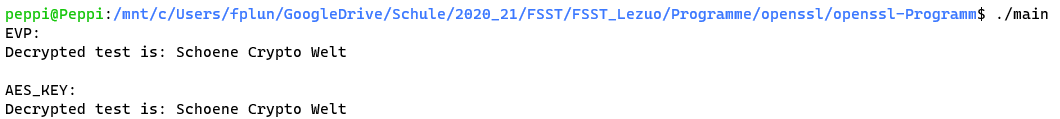
\includegraphics[width=\linewidth]{Programm-Output.png}
    \caption{Programm-Output}
    \label{caption:Programm-Output}
\end{figure}

\newpage
\section{Finales Programm als kleines Command line tool}
\lstinputlisting[language=C, style=StyleC, caption=main.c, captionpos=b, label=main.c]{../../openssl/openssl-Programm/main.c}
\lstinputlisting[language=C, style=StyleC, caption=Encryption.c, captionpos=b, label=Encryption.c]{../../openssl/openssl-Programm/Encryption.c}
\lstinputlisting[language=C, style=StyleC, caption=FileInput.c captionpos=b, label=FileInput.c]{../../openssl/openssl-Programm/FileInput.c}

\subsection{Programm Output:}
\begin{figure}[!htb]
    \centering
    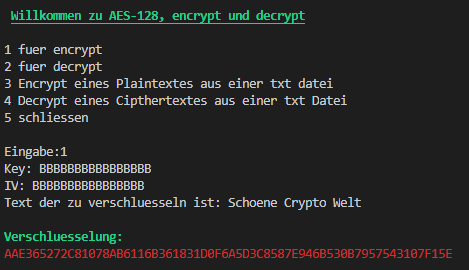
\includegraphics[scale=0.70]{Programm Output.png}
    \caption{Programm Output}
    \label{caption:Programm Output}
\end{figure}







%End------------------------------------------------------------------------------------------------------------------------------------------
%---------------------------------------------------------------------------------------------------------------------------------------------
%Codeverzeichnis
\end{document}
